% !TEX encoding = UTF-8 Unicode

\documentclass[a4paper]{article}

\usepackage{color}
\usepackage{url}
\usepackage[T2A]{fontenc} % enable Cyrillic fonts
\usepackage[utf8]{inputenc} % make weird characters work
\usepackage{graphicx}
\usepackage{listings}

\usepackage[english,serbian]{babel}

\usepackage[unicode]{hyperref}
\hypersetup{colorlinks,citecolor=green,filecolor=green,linkcolor=blue,urlcolor=blue}

%\newtheorem{primer}{Пример}[section] %ćirilični primer
\newtheorem{primer}{Primer}[section]

\begin{document}

\title{Problem Stabilnog Uparivanja\\ \small{Seminarski rad u okviru kursa\\Konstrukcija i analiza algoritama II\\ Matematički fakultet}}

\author{Rastko Đorđević, 1091/2017\\ rastko\_djordjevic@matf.bg.ac.rs}
\maketitle

\abstract{
Problem stabilnog uparivanja \textit{(eng. Stable matching problem / Stable marriage problem)} ima značaja u oblastima matematike, ekonomije i informatike. U ovom radu će biti opisan problem, algoritam za njegovo rešavanje, i implementacija datog algoritma u programskom jeziku Python.}

\tableofcontents

\newpage



\section{Postavka problema}

Kod problema stabilnog uparivanja zadatak je pronaći stabilno uparivanje između dva skupa elemenata. Za svaki element oba skupa data je lista preferenci elemenata iz suprotnog skupa. Za uparivanje kažemo da nije stabilno ako postoji element $a$ skupa A, takav da za bilo koji element $b$ skupa B koji ima veći prioritet od elementa sa kojim je A trenutno uparen važi da element $a$ takođe ima veći prioritet od elementa sa kojim je trenutno uparen element $b$. 

Ovaj problem se često formuliše kao problem stabilnog braka na sledeći način:
Za datih $n$ muškaraca i $n$ žena gde je svaka osoba ocenila sve osobe suprotnog pola, treba venčati sve muškarce i žene tako da ne postoje 2 osobe suprotnog pola koje bi radije napustile svoje trenutne partnere i oženili se jedno sa drugim. Kada ne postoji takav par osoba za skup brakova kažemo da je stabilan.

\section{Gale-Shapley algoritam}

David Gejl \textit{(eng. David Gale)} i Lojd Šepli (Lloyd Shapley) su 1962. godine dokazali da je za jednak broj muškaraca i žena uvek moguće rešiti problem stabilnog braka tako da svi brakovi budu stabilni\cite{galeShapley}. Njihov algoritam se sastoji od niza rundi:

U prvoj rundi svaki muškarac koji nije veren prosi ženu koju najviše voli. Potom svaka žena prihvata veridbu muškarca kojeg najviše voli od onih koji su je zaprosili, a ostale odbija.

U svakoj sledećoj rundi se dešava sledeće: Prvo svaki slobodan muškarac prosi ženu koju najviše voli od onih koje još nije prosio. Potom svaka žena koja nije verena prihvata veridbu muškarca kojeg najviše voli. Sve verene žene prihvataju veridbu samo ako više vole muškarca koji ih je zaprosio od trenutnog verenika i u tom slučaju ta veridba se raskida i taj verenik postaje slobodan. 

Ovaj proces se ponavlja dok svi nisu vereni. Složenost algoritma je $O(n^2)$ gde je n broj muškaraca, što su pokazali Ivama \textit{(eng. Iwama)} i Mijazaki \textit{(eng. Miyazaki)}\cite{slozenost}. 

Dati algoritam garantuje da će svi biti oženjeni. Pretpostavimo da postoje muškarac $a$ i žena $b$ koji nisu oženjeni na kraju algoritma. Muškarac je zaprosio sve žene pa samim tim i ženu $b$. Pošto $a$ i $b$ nisu oženjeni to znači da žena $b$ ili nije prihvatila njegovu prosidbu zbog nekog drugog muškarca, ili je prihvatila prosidbu pa je naknadno ostavila muškarca $b$ zbog nekog drugog muškarca. U oba slučaja žena $b$ mora biti oženjena, što je suprotno od početne pretpostavke da žena $b$ nije oženjena.

Algoritam takođe garantuje da će su svi brakovi na kraju algoritma stabilni. Pretpostavimo da postoje muškarac $a$ i žena $b$ koji su oženjeni nekim drugim osobama i koji više vole jedno drugo od svojih trenutnih partnera. Pošto muškarac $a$ više voli ženu $b$ od svoje trenutne partnerke to znači da je zaprosio ženu $b$ pre nego što je zaprosio svoju partnerku. Pošto je ženu $b$ zaprosio muškarac $a$ to znači da konačnog muškarca za kojeg se verila voli više od muškarca $a$ što je u kontradikciji sa početnom pretpostavkom da žena $b$ više voli muškarca $a$ od svog trenutnog partnera.

\newpage

Pseudo-kod algoritma:
\begin{verbatim}
Algoritam stabilno_uparivanje(M, Ž)
Ulaz:
	M - skup muškaraca M, sa uređenom listom preferiranih žena
	Ž - skup žena Ž, sa uređenom listom preferiranih muškaraca
Izlaz:
	SU - stabilno uparivanje elemenata iz skupova M i Ž
begin
    Inicijalizuj sve muškace i žene da budu slobodni
    while postoji slobodan muškarac m koji još nije zaprosio sve žene
        ž = prva žena na listi preferenci muškarca m koju m još nije zaprosio
        if ž je slobodna
            upari(m, ž)
        else neki par (m', ž) već postoji
            if ž više voli m od m'
                m' postaje slobodan
                upari(m, ž)
end
\end{verbatim}


\subsection{Optimalnost rešenja}
U opštem slučaju stabilno uparivanje nije jedinstveno stoga se postavlja pitanje kakvo rešenje vraća opisani algoritam? Da li je bolje za žene ili muškarce, ili je nešto između? Važi da su u prednosti osobe koje preuzmu inicijativu. Gejl-Šepli algoritam u kojem muškarci prose žene uvek vraća najbolje uparivanje za sve muškarce od svih mogućih stabilnih uparivanja. U suprotnom, ako bi žene prosile muškarce, onda bi rezultujuće uparivanje bilo najbolje od svih stabilnih uparivanja za sve žene. Optimalnost rešenja se može dokazati kontradikcijom.

Takođe treba razmotriti da li je algoritam moguće "prevariti"? Naime, ako bi neki muškarac znao liste prioriteta svih ostalih osoba, pitanje je da li bi mogao da promeni svoju listu prioriteta kako bi dobio voljenu ženu. Ispostavlja se da ovo nije moguće. Čak ni više muškaraca u koaliciji ne mogu da promene svoje preference tako da svi muškarci u koaliciji prođu bolje \cite{prevara}.

Sa druge strane, žene, to jest grupa koja prima prosidbe može "prevariti" algoritam. Tačnije, za žene važi da bi izmenom svoje liste preferenci mogle da dobiju boljeg muškarca nego da su bile iskrene tokom kreiranja svoje liste preferenci. 

\section{Implementacija}

Algoritam je implementiran u programskom jeziku Python. Pošto je složenost algoritma kvadratna, algoritam je upoređen sa verzijom sortiranja mehurom \textit{(eng. bubble sort)}. Kao što se može videti na grafu \ref{fig1}, izvršavanje algoritma je približno jednako izvršavanju sortiranja mehurom 5 puta. Takođe možemo primetiti da priprema podataka zahteva veliku količinu vremena i to približno 5 puta više vremena od izvršavanja samog algoritma. To je slučaj zbog izbora struktura listi preferenci, koje zahtevaju veliki broj mešanja i kopiranja ogromnih nizova. Ovo bi se moglo dodatno optimizovati ali tome nije dat ključni prioritet prilikom pisanja programa. 

Iako optimizacija nije bila najveći prioritet, uzeta je u obzir pri implementaciji algoritma. Na maksimalnom broju mesta korišćeni konstrukti u pythonu koji se direktno prevode do C koda umesto konstrukta kod kojih to nije slučaj. 


\begin{figure}
	\centering
	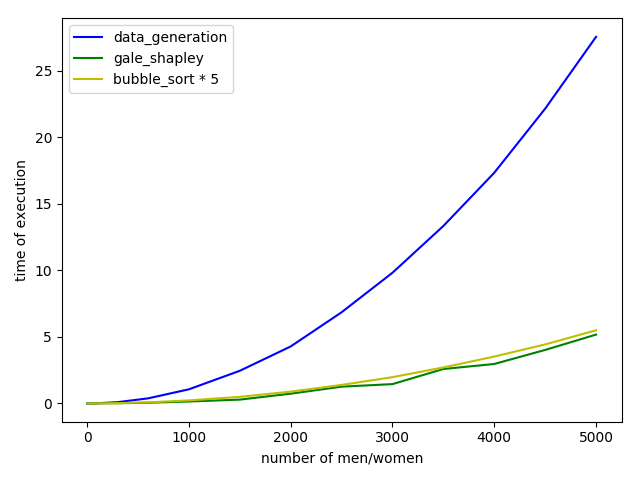
\includegraphics[scale=0.5]{resources/execution_comparison.png}
	\caption{Poređenje efikasnosti}
	\label{fig1}
\end{figure}
\section{Primene}

Algoritam za pronalazak stabilnog uparivanja se može primeniti u raznim situacijama. Najpoznatija primena je verovatno uparivanje diplomiranih studenata medicine i njihovih prvih bolnica. 

Još jedna važna primena je uparivanje korisnika interneta i servera koji distribuiraju servise. Mreže za dostavu sadržaja \textit{(eng. Content delivery networks)} koje čine ključni deo interneta izvršavaju ovaj algoritam svakih desetak sekundi kako bi omogućili svim korisnicima brz pristup željenom sadržaju.

\subsection{Praktična pitanja}
Razmatraćemo praktične probleme primene Gejl-Šepli algoritma nad problemom upisivanja studenata u univerzitete sa kojim su se i borili autori originalnog rada. Ovo je malo izmenjena verzija početnog problema, gde skup A može biti uparen sa više elemenata skupa B. Rešenje ovog problema je veoma slično već opisanom algoritmu. Nas zanima koliko je ovaj algoritam zaista upotrebljiv za spajanje studenata sa željenim univerzitetima i obratno.

Prvi očigledan problem je što algoritam zahteva dosta komunikacije napred i nazad ako bi se pratio doslovno. Jednostavno rešenje bi bilo skupiti sve liste preferenci na jedno mesto i potom izvršiti algoritam nad svim podacima. Problem sa ovim rešenjem je što bi bila neohodna ogromna količina vremena koji bi morao da uloži svaki od učesnika kako bi napravio iscrpnu listu preferenci svih univerziteta i obratno. Tako da bi se morao napraviti neki kompromis, na primer kandidati mogu poslati zahteve za samo svojih 5 omiljenih izbora.

Takođe je bitno napomenuti da nakon što je aplikant odbijen on ne mora odmah aplicirati za svoj sledeći univerzitet. Konačni izbor se neće promeniti ako aplikant preskoči narednih nekoliko rundi. Ovo znači da ceo proces neće morati da stane nakon što neki od studenata bude odbijen od svih 5 omiljenih univerziteta.

Pored tehničkih problema koji su do sada razmatrani, postoji i veliki broj problema vezanih za dodatne uslove koji nisu uzeti u obzir u algoritmu. Na primer neki studenti će pre izabrati određen univerzitet sa stipendijom ali im je previše skup bez stipendije. Neki univerziteti takođe uzimaju u obzir i ukupan sastav polazne generacije, stoga se njihove preference menjaju sa svakim primljenim studentom.

Iako se neki od pomenutih problema mogu lako rešiti izmenom algoritma, kod nekih od problema to nije slučaj. Uprkos tome što može doći do otežavajućih okolnosti pri primeni algoritma, on nam daje i neke bitne osobine. Aplikanti ne gube svoje niže izbore dok im se razmatraju omiljeni izbori. Takođe univerziteti su sigurni da aplikanti koji su na njihovoj listi čekanja nemaju druge univerzitete na koje bi radije otišli, stoga ako im se ukaže prilika prihvatiće ponudu da odu na dati univerzitet.

\addcontentsline{toc}{section}{Literatura}
\appendix
\bibliography{seminarski} 
\bibliographystyle{plain}

\end{document}
